\documentclass[a4paper,11pt]{article}
\usepackage{pdflscape}
\usepackage[utf8]{inputenc}
\usepackage[T1]{fontenc}
%\usepackage{fourier} % math & rm
%\usepackage{amsthm,amsfonts,amsmath,amssymb,textcomp}
\usepackage{pst-all,pstricks-add,pst-eucl}
\everymath{\displaystyle}
\usepackage{fp,ifthen}
%\usepackage{color}
%\usepackage{graphicx}
\usepackage{setspace}
\usepackage{array}
\usepackage{tabularx}
\usepackage{supertabular}
\usepackage{hhline}
\usepackage{variations}
\usepackage{enumerate}
\usepackage{pifont}
\usepackage{framed}
\usepackage[fleqn]{amsmath}
\usepackage{amssymb}
\usepackage[framed]{ntheorem}
\usepackage{multicol}
\usepackage{kpfonts}
\usepackage{manfnt}

%\usepackage[hmargin=2.5cm, vmargin=2.5cm]{geometry}
\usepackage{vmargin}          % Pour fixer les marges du document
\setmarginsrb
{1.5cm} 	%marge gauche
{0.5cm} 	  %marge en haut
{1.5cm}     %marge droite
{0.5cm}   %marge en bas
{1cm} 	%hauteur de l'entête
{0.5cm}   %distance entre l'entête et le texte
{1cm} 	  %hauteur du pied de page
{0.5cm}     %distance entre le texte et le pied de page

\newcommand{\R}{\mathbb{R}}
\newcommand{\N}{\mathbb{N}}
%\newcommand{\D}{\mathbb{D}}
\newcommand{\Z}{\mathbb{Z}}
\newcommand{\Q}{\mathbb{Q}}
\newcommand{\C}{\mathbb{C}}
\newcommand{\e}{\text{e}}
\newcommand{\dx}{\text{d}x}
\newcommand{\vect}[1]{\mathchoice%
  {\overrightarrow{\displaystyle\mathstrut#1\,\,}}%
  {\overrightarrow{\textstyle\mathstrut#1\,\,}}%
  {\overrightarrow{\scriptstyle\mathstrut#1\,\,}}%
  {\overrightarrow{\scriptscriptstyle\mathstrut#1\,\,}}}
\newcommand\arraybslash{\let\\\@arraycr}
\renewcommand{\theenumi}{\textbf{\arabic{enumi}}}
\renewcommand{\labelenumi}{\textbf{\theenumi.}}
\renewcommand{\theenumii}{\textbf{\alph{enumii}}}
\renewcommand{\labelenumii}{\textbf{\theenumii.}}
\renewcommand{\and}{\wedge}

\theoremstyle{break}
\theorembodyfont{\upshape}
\newcounter{enonce}
\newframedtheorem{theorem}[enonce]{Théorème}
\newframedtheorem{proposition}[enonce]{Proposition}
\newframedtheorem{definition}[enonce]{Définition}

\newtheorem{Term}{Terminologie}
\newtheorem{Rq}[enonce]{Remarque}
\newtheorem{exemple}[enonce]{Exemple}
\newtheorem{demonstration}[enonce]{Démonstration}
%\newtheorem{exo}{Exercice}

%\theorembodyfont{\small \sffamily}
%\newtheorem{sol}{solution}

\newenvironment{sol}% 
{\def\FrameCommand{\hspace{0.5cm} {\color{black} \vrule width 1pt} \hspace{-0.7cm}}%
  \framed {\advance\hsize-\width}
  \noindent \small \sffamily  %\underline{Solution :}%\\
}%
{\endframed}

\newrgbcolor{vert}{0 0.4 0}
\newrgbcolor{bistre}{1 .50 .30}
\setlength\tabcolsep{1mm}
\renewcommand\arraystretch{1.3}

\everymath{\displaystyle}
\hyphenpenalty 10000 %supprime toutes les césures
%\setcounter{secnumdepth}{0}
%\newcounter{saveenum}

\usepackage[frenchb]{babel}
%\usepackage{fancyhdr,lastpage}
%\usepackage{fancybox}

%\headheight 15.0 pt
%\fancyhead[L]{Leçon}
%\fancyhead[C]{}
%\fancyhead[R]{Chapitre 1}
%\fancyfoot[L]{{\scriptsize\textsl{Thomas Gire Cité scolaire de Lorgues}}}
%\fancyfoot[C]{\scriptsize\thepage}
%\fancyfoot[C]{\scriptsize\thepage/\pageref{LastPage}}

\title{Produit scalaire.}
\author{}
\date{}

%\pagestyle{empty}
%\pagestyle{fancy}
\usepackage[np]{numprint}

\renewcommand\arraystretch{1.8}

\newcounter{numero}
\newcommand{\exo}{
  \addtocounter{numero}{1}%
  \textbf{\underline{Exercice \arabic{numero}:}}\quad}

\frenchbsetup{StandardEnumerateEnv=true}
\usepackage{etex}
\usepackage{tikz,tkz-tab}
\usepackage{graphicx}
\graphicspath{ {../images/} }





\begin{document}
  %\setlength{\unitlength}{1mm}
  %\setlength\parindent{0mm}
 
  \maketitle


  
  \section{Angle orienté de vecteurs.}
  
  \subsection{Orientation du plan.}
  
  \begin{proposition}
   Tout cercle du plan peut être orienté en distinguant sur ce cercle deux sens de parcours. Un sens direct
   et un sens indirect.
 
 \begin{center}
   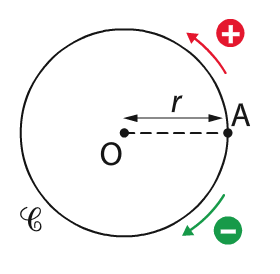
\includegraphics[scale=0.5]{../Images/orientation.png}
 \end{center}

  
   
    On peut orienter tous les cercles du plan de façon cohérente. On dit alors qu'on munit le plan lui-même
    d'une orientation. Il n'y a que deux orientations du plan possibles. Nous suivrons la convention
    qui consiste à choisir comme sens positif le sens anti-horaire (comme sur le cercle précédent).
    
    On appelle  \textbf{cercle trigonométrique} un cercle orienté de rayon $1$. 
    
  \end{proposition}

   

  
  \subsection{Angle orienté de vecteurs.}
 
  \begin{definition}
  
  Soient $\vec{u}$ et $\vec{v}$ deux vecteurs non nuls. Soit $\mathcal{C}$ un cercle trigonométrique de 
  centre $O$, $A$ et $B$ les uniques points sur le cercle trigonométrique tels que $\vec{OA}$ 
  (resp. $\vec{OB}$) est colinéaire à $\vec{u}$ (resp. $\vec{v}$).
  
  On note $l$ la longueur de l'arc $\wideparen{AB}$ parcouru dans le sens direct ($l \geq 0$).
  
  \begin{center}
    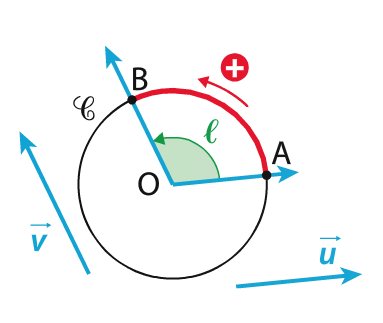
\includegraphics[scale=0.5]{../Images/angleOriente.png}
  \end{center}
  
  Au couple $(\vec{u},\vec{v})$, on associe la famille de nombres réels de la forme 
  $l+2k\pi, k \in \mathbb{Z}$. Chacun de ces nombres est une mesure de l'\textbf{angle orienté}
   de vecteurs $(\vec{u},\vec{v})$.
   
   L'usage est de noter $(\vec{u},\vec{v})$ un angle de vecteurs et de confondre un angle avec l'une
   de ses mesures. On appelle \textbf{radian} l'unité de mesure des angles orientés de vecteurs.

  
  \end{definition}
 
  \newpage
 
 \subsection{Mesure principale d'un angle orienté.}
 
 \begin{definition}
  \begin{itemize}
   \item Parmi les mesures $x+2k\pi$ de l'angle orienté $(\vec{u},\vec{v})$ de deux vecteurs non nuls,
   il en existe une et une seule dans l'intervalle $]-\pi;\pi]$. Cette mesure est 
   apellée la \textbf{mesure 
   principale} de $(\vec{u},\vec{v})$.
   \item On appelle mesure de l'\textbf{angle géométrique} défini par $\vec{u}$ et $\vec{v}$ la valeur
   absolue de la mesure principale de $(\vec{u},\vec{v})$.
  \end{itemize}

 \end{definition}

 \begin{exemple} \vspace{0.1cm}~
 
 \begin{itemize}
  \item $\frac{37}{6}\pi=(6+\frac{1}{6})\pi=\frac{\pi}{6}+3(2\pi)$. La mesure principale est $\frac{\pi}{6}$.
  \item $\frac{202\pi}{3}=(67+\frac{1}{3})\pi=\frac{\pi}{3}+67\pi=68\pi - \pi+\frac{\pi}{3}=-\frac{2\pi}{3}
  +34(2\pi)$. La mesure principale est donc $-\frac{2\pi}{3}$. L'angle géométrique associé a pour mesure
  $|-\frac{2\pi}{3}|=\frac{2\pi}{3}$.
  \item Les mesures des angles géométriques en degré et en radian sont proportionnels:
  
  \renewcommand{\arraystretch}{2.2}
 $$
\begin{array}{|c|c|c|c|c|}

\hline
    deg.&180&90&60&30\\
    \hline
    rad.&\pi&\frac{\pi}{2}&\frac{\pi}{3}&\frac{\pi}{6}\\
    \hline
    \end{array} 
$$  
 \end{itemize}

 
 \end{exemple}
 
 \section{Propriétés des angles orientés.}
 
 \subsection{Colinéarité.}
 
 \begin{theorem}
 Soient $\vec{u}$ et $\vec{v}$ deux vecteurs non nuls.
  \begin{itemize}
   \item $(\vec{u},\vec{v})=0$ si et seulement si les vecteurs $\vec{u}$ et $\vec{v}$ sont colinéaires
   et de même sens.
   \begin{center}
      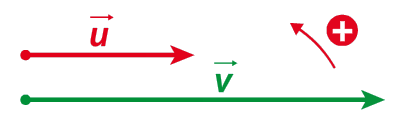
\includegraphics[scale=0.5]{../Images/colMemeSens.png}
   \end{center}

   
   \item $(\vec{u},\vec{v})=\pi$ si et seulement si les vecteurs $\vec{u}$ et $\vec{v}$ sont colinéaires
   et de sens contraires.
   \begin{center}
      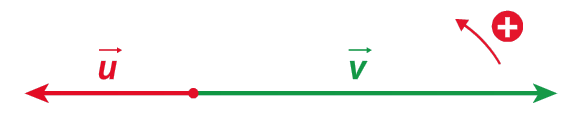
\includegraphics[scale=0.5]{../Images/colSensContraire.png}
   \end{center}
   
  \end{itemize}

 \end{theorem}
 
 \subsection{Orthogonalité.}
 
 \begin{definition}
 ~\vspace{-0.5cm}
 
   Les vecteurs $\vec{u}$ et $\vec{v}$ sont \textbf{orthogonaux} si
   $(\vec{u},\vec{v})=\frac{\pi}{2}$ ou $(\vec{u},\vec{v})=-\frac{\pi}{2}$.
   \begin{center}
      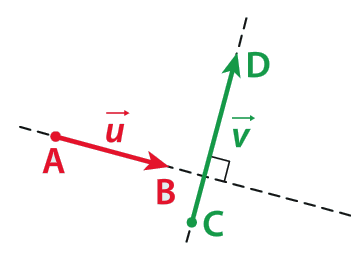
\includegraphics[scale=0.5]{../Images/Ortho.png}
   \end{center}

 \end{definition}

 \subsection{Relation de Chasles.}
 
 \begin{theorem}
  Pour tous vecteurs non nuls $\vec{u}$, $\vec{v}$ et $\vec{w}$, on a 
  $(\vec{u},\vec{v})+(\vec{v},\vec{w})=(\vec{u},\vec{w})$.
 \end{theorem}
 
 \begin{exemple}
 \begin{multicols}{2} 
 
  Avec la figure ci-contre:   
  
   $(\vec{BA},\vec{CD})=(\vec{BA},\vec{BC})+(\vec{BC},\vec{CD})$
   
   d'où $(\vec{BA},\vec{CD})=-\frac{3\pi}{4}+\frac{\pi}{3}=\frac{5\pi}{12}$.
   
   \columnbreak 
   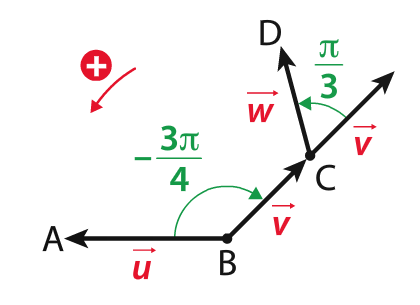
\includegraphics[scale=0.5]{../Images/relChasles.png}
  \end{multicols}

 \end{exemple}
\begin{proposition}
 Pour tous vecteurs non nuls $\vec{u}$ et $\vec{v}$:
 \begin{multicols}{2}
  
  
  \begin{center}
    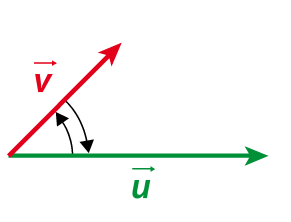
\includegraphics[scale=0.5]{../Images/moinsuv.png}
  \end{center}
  $$(\vec{v},\vec{u})=-(\vec{u},\vec{v})$$
  
  \columnbreak 
  
  
  \begin{center}
    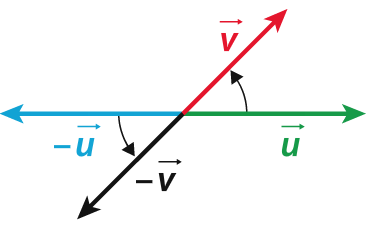
\includegraphics[scale=0.5]{../Images/moinsUetmoinsV.png}
  \end{center}
  $$(-\vec{u},-\vec{v})=(\vec{u},\vec{v})$$
  
  \end{multicols}
  

  
\end{proposition}

\begin{proposition}
 Pour tous vecteurs non nuls $\vec{u}$ et $\vec{v}$:
 \begin{multicols}{2}
  
  \begin{center}
    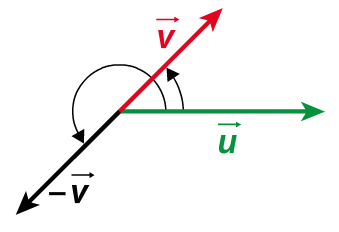
\includegraphics[scale=0.5]{../Images/uMoinsv.png}
  \end{center}
  $$(\vec{u},-\vec{v})=(\vec{u},\vec{v})+\pi$$
  
  \columnbreak 

    \begin{center}
    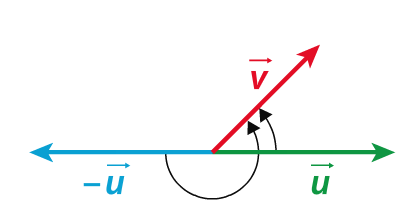
\includegraphics[scale=0.5]{../Images/moinsUetV.png}
  \end{center}
  $$(-\vec{u},\vec{v})=(\vec{u},\vec{v})+\pi$$
  \end{multicols}
\end{proposition}

\begin{proposition}
Pour tous vecteurs non nuls $\vec{u}$ et $\vec{v}$
et $k,l>0$, $(k\vec{u},l\vec{v})=(\vec{u},\vec{v})$
 \begin{center}
    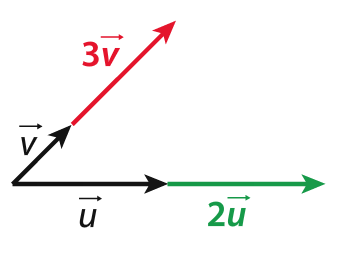
\includegraphics[scale=0.5]{../Images/2u3v.png}
  \end{center}
\end{proposition}





\newpage
 
  \section{Produit scalaire.}
 
 \subsection{Norme d'un vecteur.}
 
 \begin{definition}
  Une unité de longueur étant choisie, on appelle \textbf{norme} d'un vecteur $\vec{u}=\vec{AB}$
  la longueur $AB$. On note $\|\vec{u}\|=\|\vec{AB}\|=AB$.
 \end{definition}

 \subsection{Repères orthonormés directs.}
 
 \begin{definition}
  Une unité de longueur étant choisie, dans le plan orienté, on dit que le repère $(O;\vec{i},\vec{j})$
  est \textbf{orthonormé direct} si $\| \vec{i} \|=\| \vec{j}\|=1$ et $(\vec{i},\vec{j})=\frac{\pi}{2}$.
  
  Dans un repère orthonormé, si $\vec{u}$ a pour coordonnées $(x;y)$ alors $\|\vec{u}\|=\sqrt{x^2+y^2}$.
  
   \begin{center}
    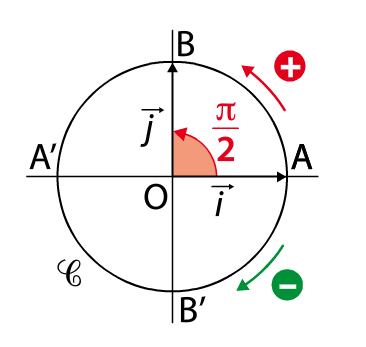
\includegraphics[scale=0.5]{../Images/repereOrthoDirect.png}
  \end{center}
  
 \end{definition}

 \subsection{Trigonométrie.}
 \begin{definition}
 Soient $a$ un angle orienté de vecteurs et $(O;\vec{OA},\vec{OB})$ un repère orthonormé direct. 
 Le \textbf{cosinus} et le \textbf{sinus} de $a$ sont les coordonnées du point $M$ sur un cercle trigonométrique de centre $O$
 tel que $(\vec{OA},\vec{OM})=a$.
  \begin{multicols}{2}
  
  
  \begin{center}
    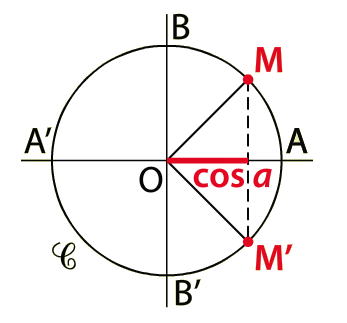
\includegraphics[scale=0.5]{../Images/cosinus.png}
  \end{center}
  
  \columnbreak 
  
  
  \begin{center}
    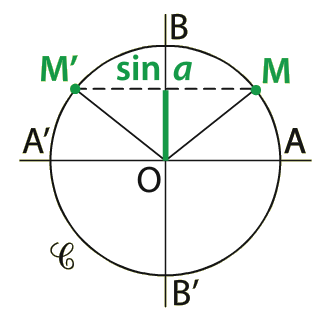
\includegraphics[scale=0.5]{../Images/sinus.png}
  \end{center}

  \end{multicols}
  \begin{center}
   $cos^2(a)+sin^2(a)=1$
  \end{center}

 \end{definition}
 
 \newpage
 
 \subsection{Définitions du produit scalaire.}
 
 \begin{definition}
  Le \textbf{produit scalaire} de deux vecteurs $\vec{u}$ et $\vec{v}$ est un nombre réél. On le note
  $\vec{u}.\vec{v}$ et on lit $\vec{u}$ <<scalaire>> $\vec{v}$. Les définitions suivantes sont équivalentes:
  
  \begin{enumerate}
   \item $\vec{u}.\vec{v}=\frac{1}{2}(\|u+v\|^2-\|\vec{u}\|^2-\|\vec{v}\|^2)$.
   \item $\vec{u}.\vec{v}=\|\vec{u}\|\times\|\vec{v}\|\times cos(\vec{u},\vec{v})$ si $\vec{u}$ et $\vec{v}$ sont non nuls.
   \item $\vec{u}.\vec{v}=xx'+yy'$ si $\vec{u}(x;y)$ et $\vec{v}(x';y')$ dans un repère orthonormé.
  \end{enumerate}
  
 \end{definition}
 
 \subsection{Règles de calcul.}
 
 Le produit scalaire possède les mêmes propriétés de calcul que le produit de nombres rééls:
 \begin{proposition}
  \begin{enumerate}
   \item Commutativité: $\vec{u}.\vec{v}=\vec{v}.\vec{u}$
   \item Distributivité: $\vec{u}.(\vec{v}+\vec{w})=\vec{u}.\vec{v}+\vec{u}.\vec{w}$
   \item <<Associativité>>: $(a\vec{u}).(b\vec{v})=(ab)\vec{u}.\vec{v}$
  \end{enumerate}

 \end{proposition}

   
  \begin{exemple}

  \vspace{0.5cm}~
  
  \begin{tabular}{c c}
  \begin{minipage}[b]{0.47\textwidth}

 $(-\vec{u}).\vec{v}=-\vec{u}.\vec{v}$
 
 $(\vec{u}+\vec{v})^2=\vec{u}^2+\vec{v}^2+2\vec{u}.\vec{v}$
 
 $(\vec{u}-\vec{v})^2=\vec{u}^2+\vec{v}^2-2\vec{u}.\vec{v}$
 
 $(\vec{u}+\vec{v})(\vec{u}-\vec{v})=\vec{u}^2-\vec{v}^2$

  \end{minipage}
&
  \begin{minipage}[b]{0.47\textwidth}
   
 
 $\vec{AB}.\vec{CD}=-\vec{BA}.\vec{CD}=-\vec{AB}.\vec{DC}=\vec{BA}.\vec{DC}$
 
  $(\vec{AB}+\vec{CD})^2=AB^2+CD^2+2\vec{AB}.\vec{CD}$
  
  $(\vec{AB}-\vec{CD})^2=AB^2+CD^2-2\vec{AB}.\vec{CD}$
  
  $(\vec{AB}+\vec{CD})(\vec{AB}-\vec{CD})=AB^2-CD^2$


  \end{minipage}

  \end{tabular}

  \end{exemple}

\subsection{Produit scalaire et orthogonalité.} 

\begin{theorem}

 Deux vecteurs $\vec{u}$ et $\vec{v}$ non nuls sont orthogonaux si et seulement si $\vec{u}.\vec{v}=0$. De même, deux droites $(AB)$ et $(CD)$ sont perpendiculaires si et seulement si $\vec{AB}.\vec{CD}=0$.
\end{theorem}

\begin{proposition}
 Soient $\vec{AB}$ et $\vec{CD}$ deux vecteurs non nuls et $C'$, (resp. $D'$)
 le projeté orthogonal de $C$ (resp. $D$) sur la droite $(AB)$. On a 
 $$\vec{AB}.\vec{CD}=\vec{AB}.\vec{C'D'}$$
 
   \begin{center}
    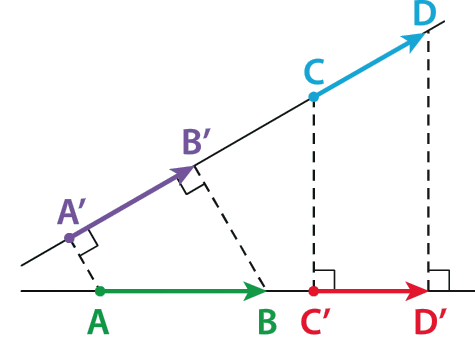
\includegraphics[scale=0.5]{../Images/projetes.png}
  \end{center}
 
 
\end{proposition}
  
 \newpage

 \section{\'Equations de droites.}
 
 \subsection{Vecteur normal à une droite.}
 
 \begin{definition}
  Un vecteur non nul $\vec{n}$ est \textbf{normal} à une droite $d$ si il est orthogonal à tout vecteur
  directeur de $d$.
  
 \end{definition}
 
 \begin{proposition}
  Un point $M$ appartient à la droite $d$ passant par $A$ et perpendiculaire à la droite $(PQ)$
  si et seulement si $\vec{AM}.\vec{PQ}=0$
  
     \begin{center}
    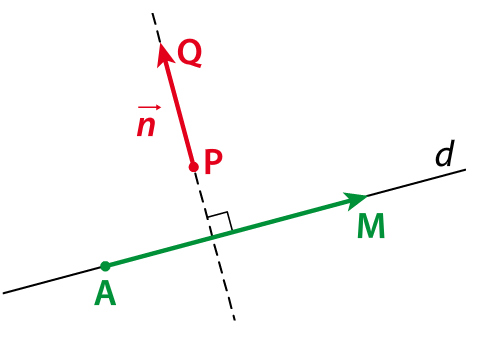
\includegraphics[scale=0.5]{../Images/vecNormal.png}
  \end{center}
  
  Si $d$ et $d'$ sont deux droites de vecteurs directeurs respectifs $\vec{u}$ et $\vec{u'}$ et 
  de vecteurs normaux respectifs $\vec{n}$ et $\vec{n'}$ alors
  $$ d \perp d' \Leftrightarrow \vec{u}.\vec{u'}=0 \Leftrightarrow \vec{n}.\vec{n'}=0$$
 \end{proposition}
 
 \begin{theorem}
  Dans un repère orthonormé:
  \begin{enumerate}
   \item Si une droite $d$ possède une équation de la forme $ax+by+c=0$ avec $a \neq0$ ou
   $b \neq 0$ alors $\vec{n}(a,b)$ est un vecteur normal de $d$.
   \item Si un vecteur $\vec{n}(a;b) \neq \vec{0}$ est normal à une droite $d$ alors
   $d$ possède une équation de la forme $ax+by+c=0$.
  \end{enumerate}

 \end{theorem}
 
 \begin{exemple}
  Soient $A(1;2)$, $B(2;5)$ et $C(4;2)$ dans un repère orthonormé. Trouver une équation 
  cartésienne pour la droite $d$ perpendiculaire à $(AB)$ passant par $C$.
  
  $\vec{AB}(1;3)$ est un vecteur normal à $d$. $d$ possède une équation de la forme $d:x+3y+c=0$.
  $C(4;2) \in d \Leftrightarrow 4+3 \times 2+c=0 \Leftrightarrow c=-10$. En définitive,
  $d:x+3y-10=0$.
 \end{exemple}


\newpage

\section{\'Equations de cercles.}

\begin{theorem}
 Dans un repère orthonormé, le cercle $\mathcal{C}$ de centre $I(x_0;y_0)$ et de rayon $r$ a
 pour équation $$\mathcal{C}:(x-x_0)^2+(y-y_0)^2=r^2$$
 
      \begin{center}
    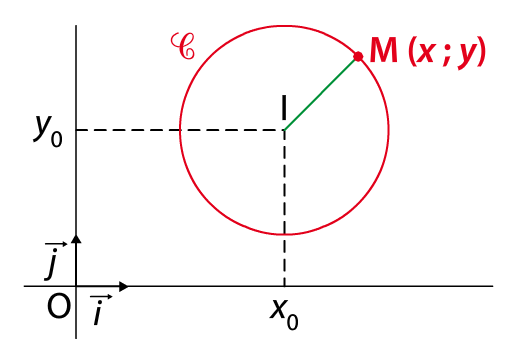
\includegraphics[scale=0.5]{../Images/cercleCentreI.png}
  \end{center}
\end{theorem}

\begin{demonstration}
 $M(x;y) \in \mathcal{C} \Leftrightarrow IM^2=r^2 \Leftrightarrow (x-x_0)^2+(y-y_0)^2=r^2$
\end{demonstration}

\begin{exemple}
 $(x+1)^2+(y-2)^2=12$ est l'équation d'un cercle de centre $I(-1;2)$ et de rayon $r=2\sqrt{3}$.
\end{exemple}

\begin{theorem}
 $M$ appartient au cercle de diamètre $[AB]$ si et seulement si $\vec{AM}.\vec{BM}=0$.
 
      \begin{center}
    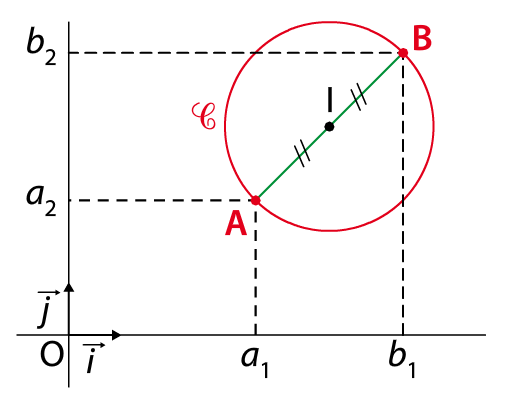
\includegraphics[scale=0.5]{../Images/cercleDiametre.png}
  \end{center}
\end{theorem}

\begin{demonstration}
 Dans un repère orthonormé, $M(x;y)$, $A(a_1;a_2)$ et $B(b_1;b_2)$.
 
 $\vec{MA}.\vec{MB}=0 \Leftrightarrow (x-a_1)(x-b_1)+(y-a_2)(y-b_2)=0$
 
 $\Leftrightarrow [x^2-(a_1+b_1)x]+[y^2-(a_2+b_2)y]=-a_1b_1-a_2b_2$
 
 $\Leftrightarrow [(x-\frac{a_1+b_1}{2})^2-(\frac{a_1+b_1}{2})^2]+[(y-\frac{a_2+b_2}{2})^2-(\frac{a_2+b_2}{2})^2]=-a_1b_1-a_2b_2$
 
 $\Leftrightarrow (x-x_I)^2+(y-y_I)^2=\frac{1}{4}[(a_1+b_1)^2+(a_2+b_2)^2-4a_1b_1-4a_2b_2]=(\frac{1}{2}[(b_1-a_1)]^2+\frac{1}{2}[(b_2-a_2)]^2)=(\frac{AB}{2})^2$
\end{demonstration}

\begin{demonstration}[Sans coordonnées]
 $\vec{MA}.\vec{MB}=0 \Leftrightarrow (\vec{MI}+\vec{IA}).(\vec{MI}+\vec{IB})=0$ où I est le milieu de $[AB]$.
 
 $\Leftrightarrow (\vec{MI}+\vec{IA}).(\vec{MI}-\vec{IA})=0$
 
 $\Leftrightarrow \vec{MI}^2-\vec{IA}^2=0$
 
 $\Leftrightarrow MI^2-IA^2=0$
 
 $\Leftrightarrow MI=IA$
\end{demonstration}



\newpage

\subsection{Théorème de Pythagore généralisé.}

\begin{theorem}
 Soit $ABC$ un triangle quelconque. $BC^2=AB^2+AC^2-2 \times AB\times AC\times cos(\vec{AB};\vec{AC})$.
 
\end{theorem}

\begin{demonstration}
 $BC^2=\vec{BC}^2=(\vec{AC}-\vec{AB})^2=AB^2+AC^2-2\times AB\times AC \times cos(\vec{AB};\vec{AC})$
\end{demonstration}


\subsection{Théorème de la médiane.}

\begin{theorem}
 Soit $ABC$ un triangle quelconque et $I$ le milieu de $[BC]$. $AB^2+AC^2=2AI^2+\frac{BC^2}{2}$
 
   \begin{center}
    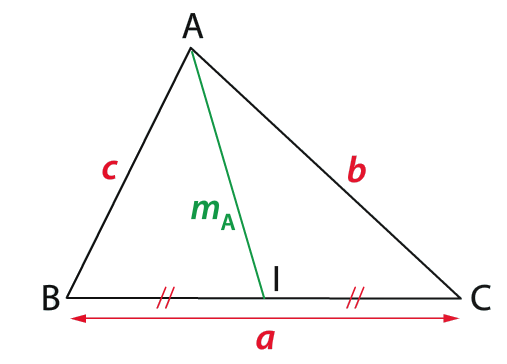
\includegraphics[scale=0.5]{../Images/mediane.png}
  \end{center}
\end{theorem}

\begin{demonstration}
 $AB^2+AC^2=(\vec{AI}+\vec{IB})^2+(\vec{AI}+\vec{IC})^2=
 2AI^2+2IB^2+2(\vec{AI}.\vec{IB}+\vec{AI}.\vec{IC})=
 2AI^2+\frac{BC^2}{2}$. 
 
 En effet, $\vec{AI}.\vec{IB}+\vec{AI}.\vec{IC}=\vec{AI}.(\vec{IB}+\vec{IC})=\vec{AI}.\vec{0}=0$.
\end{demonstration}


\subsection{Formules trigonométriques}

\begin{theorem}
~

 Formules d'addition:
 
 $sin(a+b)=sin(a)cos(b)+cos(a)sin(b)$
 
 $cos(a+b)=cos(a)cos(b)-sin(a)sin(b)$
 
 $sin(a-b)=sin(a)cos(b)-cos(a)sin(b)$
  
 $cos(a-b)=cos(a)cos(b)+sin(a)sin(b)$
 \vspace{0.5cm}
 
 Formules de duplication:
 
 $cos(2a)=cos^2(a)-sin^2(a)=2cos^2(a)-1=1-2sin^2(a)$
 
 $sin(2a)=2sin(a)cos(a)$
 \vspace{0.5cm}
 
 Formules de linéarisation:
  
 $cos^2(a)=\frac{1+cos(2a)}{2}$
 
 $sin^2(a)=\frac{1-cos(2a)}{2}$
\end{theorem}
   
\end{document}